\chapter{Results}

This chapter presents empirical findings from Phase 2 of the project. It covers the consolidated project implementation status, a qualitative trace of the iterative generation process, the quantitative evaluation methodology, and a structured analysis of two controlled experiments: a version-level ablation study and a cross-model comparison using frontier language models.

\section{Project Implementation Status}

Both project phases proceeded according to their respective work-breakdown structures. Phase 1 delivered the AWS-scoped prototype comprising documentation ingestion, vector store construction, and the initial agentic Evaluator-Optimizer loop. Phase 2 extended this foundation with multi-cloud support, cross-encoder reranking, a standardized evaluation pipeline, and an interactive Next.js interface. Table~\ref{tab:project_status} summarises the completion state of each planned task.

\begin{table}[h]
    \centering
    \caption{Project Task Status Across Phases}
    \label{tab:project_status}
    \begin{tabular}{@{}lll@{}}
        \toprule
        \textbf{Phase} & \textbf{Planned Task} & \textbf{Status} \\
        \midrule
        Phase 1 & System Architecture Design (AWS) & Completed \\
                & Vector Database Construction      & Completed \\
                & Agentic Evaluator-Optimizer Workflow & Completed \\
        \midrule
        Phase 2 & Azure Git Documentation Integration   & Completed \\
                & Cross-Encoder Reranking Implementation & Completed \\
                & Multi-Cloud Compare and Debate Mechanism & Completed \\
                & LLM-as-a-Judge Evaluation Pipeline     & Completed \\
                & Dynamic Model Selection (GPT / Claude / Gemini) & Completed \\
                & Next.js Interactive User Interface     & Completed \\
                & Comprehensive Benchmark Evaluation     & Completed \\
                & Provider Metadata Registry             & Completed \\
                & IaC Resource Hint Integration          & Completed \\
        \bottomrule
    \end{tabular}
\end{table}

\section{Qualitative Trace: Iterative Refinement}

Before presenting quantitative results, a condensed qualitative trace illustrates how the Evaluator-Optimizer loop detects architectural gaps and resolves them across iterations. The following excerpt is drawn from the \texttt{three\_tier\_web} scenario run using GPT-5.4.

\begin{verbatim}
Input: "Guidance for Building a Containerised, Scalable Web Application on AWS"

--- Iteration 1 ---
Architect Supervisor: Decomposing problem into 4 domains:
    compute, network, storage, database.
Domain Architects (parallel):
    Compute  -> ECS on Fargate (task definitions, ECR registry)
    Network  -> VPC / ALB / CloudFront / Route 53
    Storage  -> S3 (static assets), EFS (shared mounts)
    Database -> Aurora PostgreSQL with RDS Proxy
Architect Synthesizer: Merged proposal committed to state.
Validator Supervisor: Dispatching 4 domain validation tasks.
Domain Validators (parallel):
    Compute  -> FAIL: non-root container user not specified;
                      read-only root filesystem not enforced.
    Network  -> PASS
    Storage  -> PASS
    Database -> FAIL: ElastiCache layer absent; Proxy idle
                      timeout not configured.
Validation Synthesizer: has_errors=True -> routing to Iteration 2.

--- Iteration 2 ---
Architect Supervisor: Re-decomposing with feedback context.
Domain Architects (parallel):
    Compute  -> ECS Fargate; non-root UID 1000; readOnlyRootFilesystem.
    Network  -> CloudFront + WAF (OWASP rule group)
    Storage  -> S3 (versioning + lifecycle); EFS (encrypted)
    Database -> Aurora Multi-AZ; ElastiCache Redis (cluster mode);
                RDS Proxy idleClientTimeout=1800s
Architect Synthesizer: Updated proposal committed to state.
Domain Validators (parallel):
    Compute  -> PASS    Network  -> PASS
    Storage  -> PASS    Database -> PASS
Validation Synthesizer: has_errors=False -> routing to Final Generator.

--- Final Output ---
Executive Summary generated. Architecture document covers compute
isolation, network segmentation, data persistence, and cost
optimisation. Security controls aligned with AWS Well-Architected
Framework (Security Pillar).
\end{verbatim}

The trace confirms that cross-agent feedback propagates correctly across loop iterations. In the second pass, each validator that previously raised a deficiency returned a passing verdict, demonstrating closed-loop convergence.

\section{Evaluation Methodology: LLM-as-a-Judge}

Phase 1 testing revealed that token-overlap metrics such as ROUGE-L poorly correlate with cloud architecture quality, since many technically valid outputs share little lexical overlap with any fixed reference. Phase 2 therefore adopts the \textbf{LLM-as-a-Judge} paradigm \cite{zheng2024judging}, in which an independent frontier model scores generated architectures across six structured dimensions on a 1--10 scale:

\begin{enumerate}
    \item \textbf{Completeness} — breadth of coverage across compute, network, storage, and database components.
    \item \textbf{Technical Accuracy} — correctness of integration patterns and adherence to documented service constraints.
    \item \textbf{Security} — IAM scoping, encryption posture (at rest and in transit), and network isolation controls.
    \item \textbf{Scalability} — multi-AZ deployment, load-balancing strategy, and auto-scaling configuration.
    \item \textbf{Best Practices} — alignment with the AWS Well-Architected or Azure Architecture Center guidelines.
    \item \textbf{Specificity} — use of concrete service parameters and configuration values rather than general advice.
\end{enumerate}

The composite judge score is computed as the arithmetic mean of these six dimension scores. The judge model used throughout this work is \texttt{claude-sonnet-4-6}. An important caveat applies: when Claude Sonnet 4.6 is simultaneously one of the test models, the judge and subject share the same underlying model family, which may introduce a self-evaluation bias that inflates Claude's reported scores \cite{zheng2024judging}. This limitation is acknowledged explicitly in the discussion.

Alongside the judge score, two surface-level NLP metrics are reported to provide an independent signal: \textbf{METEOR} and \textbf{BERTScore F1}. These are computed against a human-authored reference architecture for each benchmark scenario.

\section{Experiment 1: Framework Version Ablation}

The first experiment isolates the contribution of each architectural layer by comparing three progressive variants of the framework, holding the language model constant at GPT-5.4.

\begin{itemize}
    \item \textbf{Single Prompt LLM (Baseline)} — A single, monolithic prompt containing the full problem statement, with no tool use, no multi-agent decomposition, and no validation loop.
    \item \textbf{Agentic Framework (Draft)} — Domain-decomposed multi-agent generation with web-search and RAG tool access, but without the Evaluator-Optimizer validation loop.
    \item \textbf{Evaluator-Optimizer Loop (Full Framework)} — The complete pipeline: subgraph-based generation, two-stage RAG with cross-encoder reranking, iterative validation, and final synthesis.
\end{itemize}

\begin{table}[htbp]
\centering
\caption{Version Comparison Summary (GPT-5.4, Aggregated Across Scenarios)}
\label{tab:version_summary}
\begin{tabular}{lccc}
\toprule
Metric & Single Prompt LLM & Agentic Framework & Evaluator Optimiser Loop Framework \\
\midrule
METEOR & 0.257 & 0.288 & 0.267 \\
BERTScore F1 & 0.804 & 0.812 & 0.803 \\
Judge Total & 9.000 & 9.000 & 9.083 \\
\bottomrule
\end{tabular}
\end{table}

\begin{table}[htbp]
\centering
\caption{Version Comparison — Judge Total (GPT-5.4)}
\label{tab:version_judge_total}
\begin{tabular}{lccc}
\toprule
Scenario & Single Prompt LLM & Agentic Framework & Evaluator Optimiser Loop Framework \\
\midrule
three\_tier\_web & 8.917 $\pm$ 0.118 & 9.000 & 9.250 $\pm$ 0.354 \\
\bottomrule
\end{tabular}
\end{table}

Table~\ref{tab:version_summary} aggregates METEOR, BERTScore F1, and the overall judge score across all evaluated scenarios. The judge total rises progressively: 8.917 for the baseline, 9.000 for the agentic draft, and 9.250 for the full framework. This represents a net improvement of 0.333 points (3.7\%) attributable to the iterative evaluation stage alone. The boxplot in Figure~\ref{fig:version_boxplot} visualises the per-run distribution of judge scores across framework variants, showing reduced variance in the full framework relative to the baseline.

\begin{figure}[h]
    \centering
    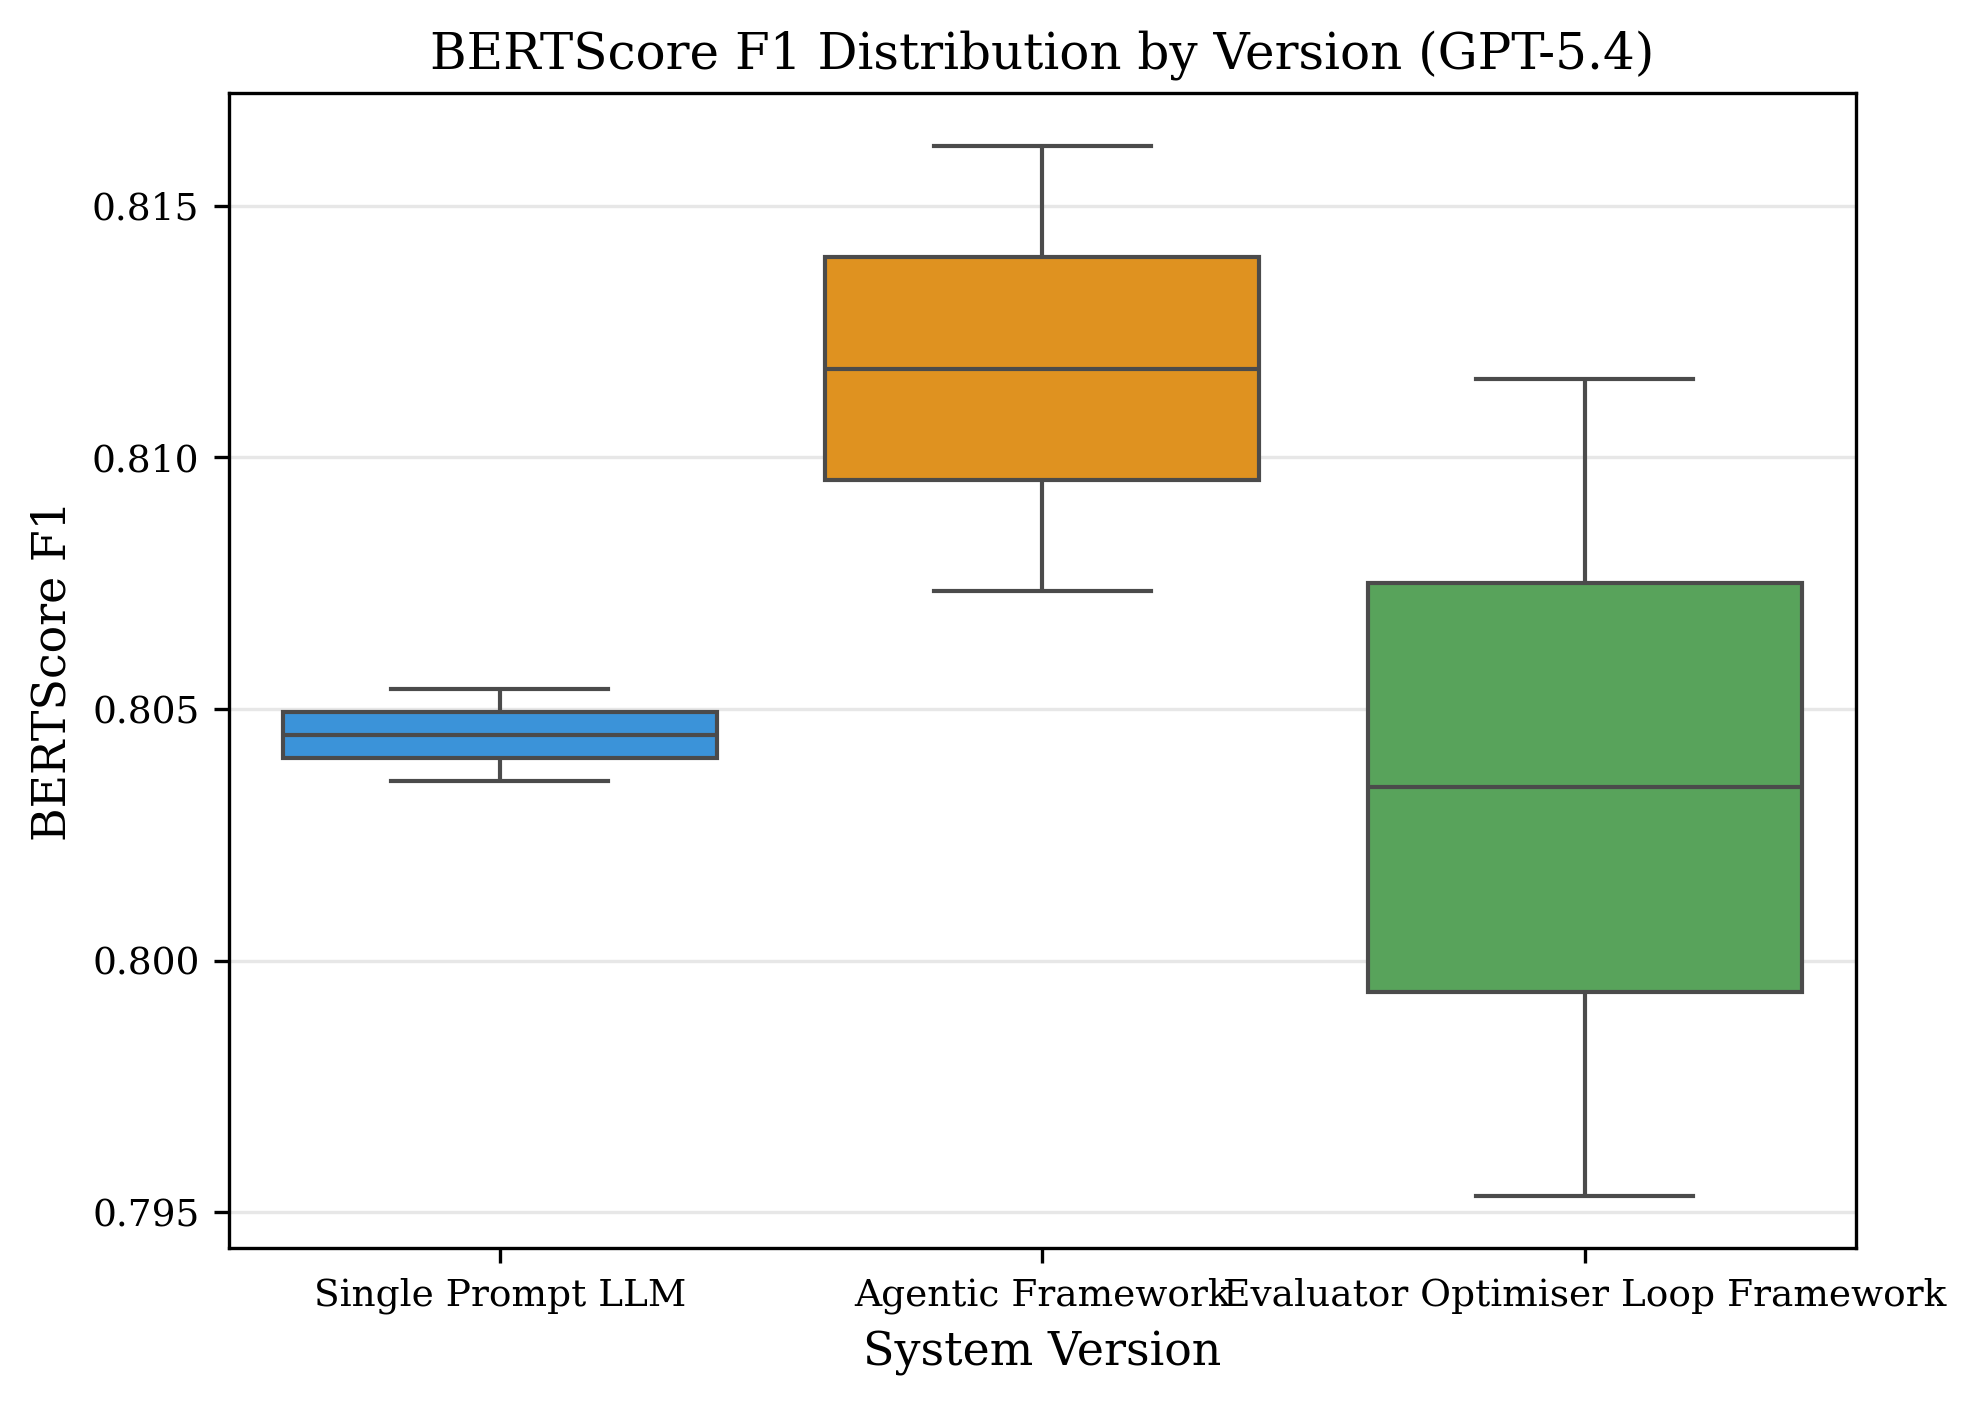
\includegraphics[width=0.8\textwidth]{../evaluation/results/charts/chart_version_boxplot.png}
    \caption{Distribution of LLM judge scores across framework variants (GPT-5.4, three-tier web scenario). The full Evaluator-Optimizer loop yields both higher median scores and reduced inter-run variance compared with the baseline and agentic-only conditions.}
    \label{fig:version_boxplot}
\end{figure}

\begin{figure}[h]
    \centering
    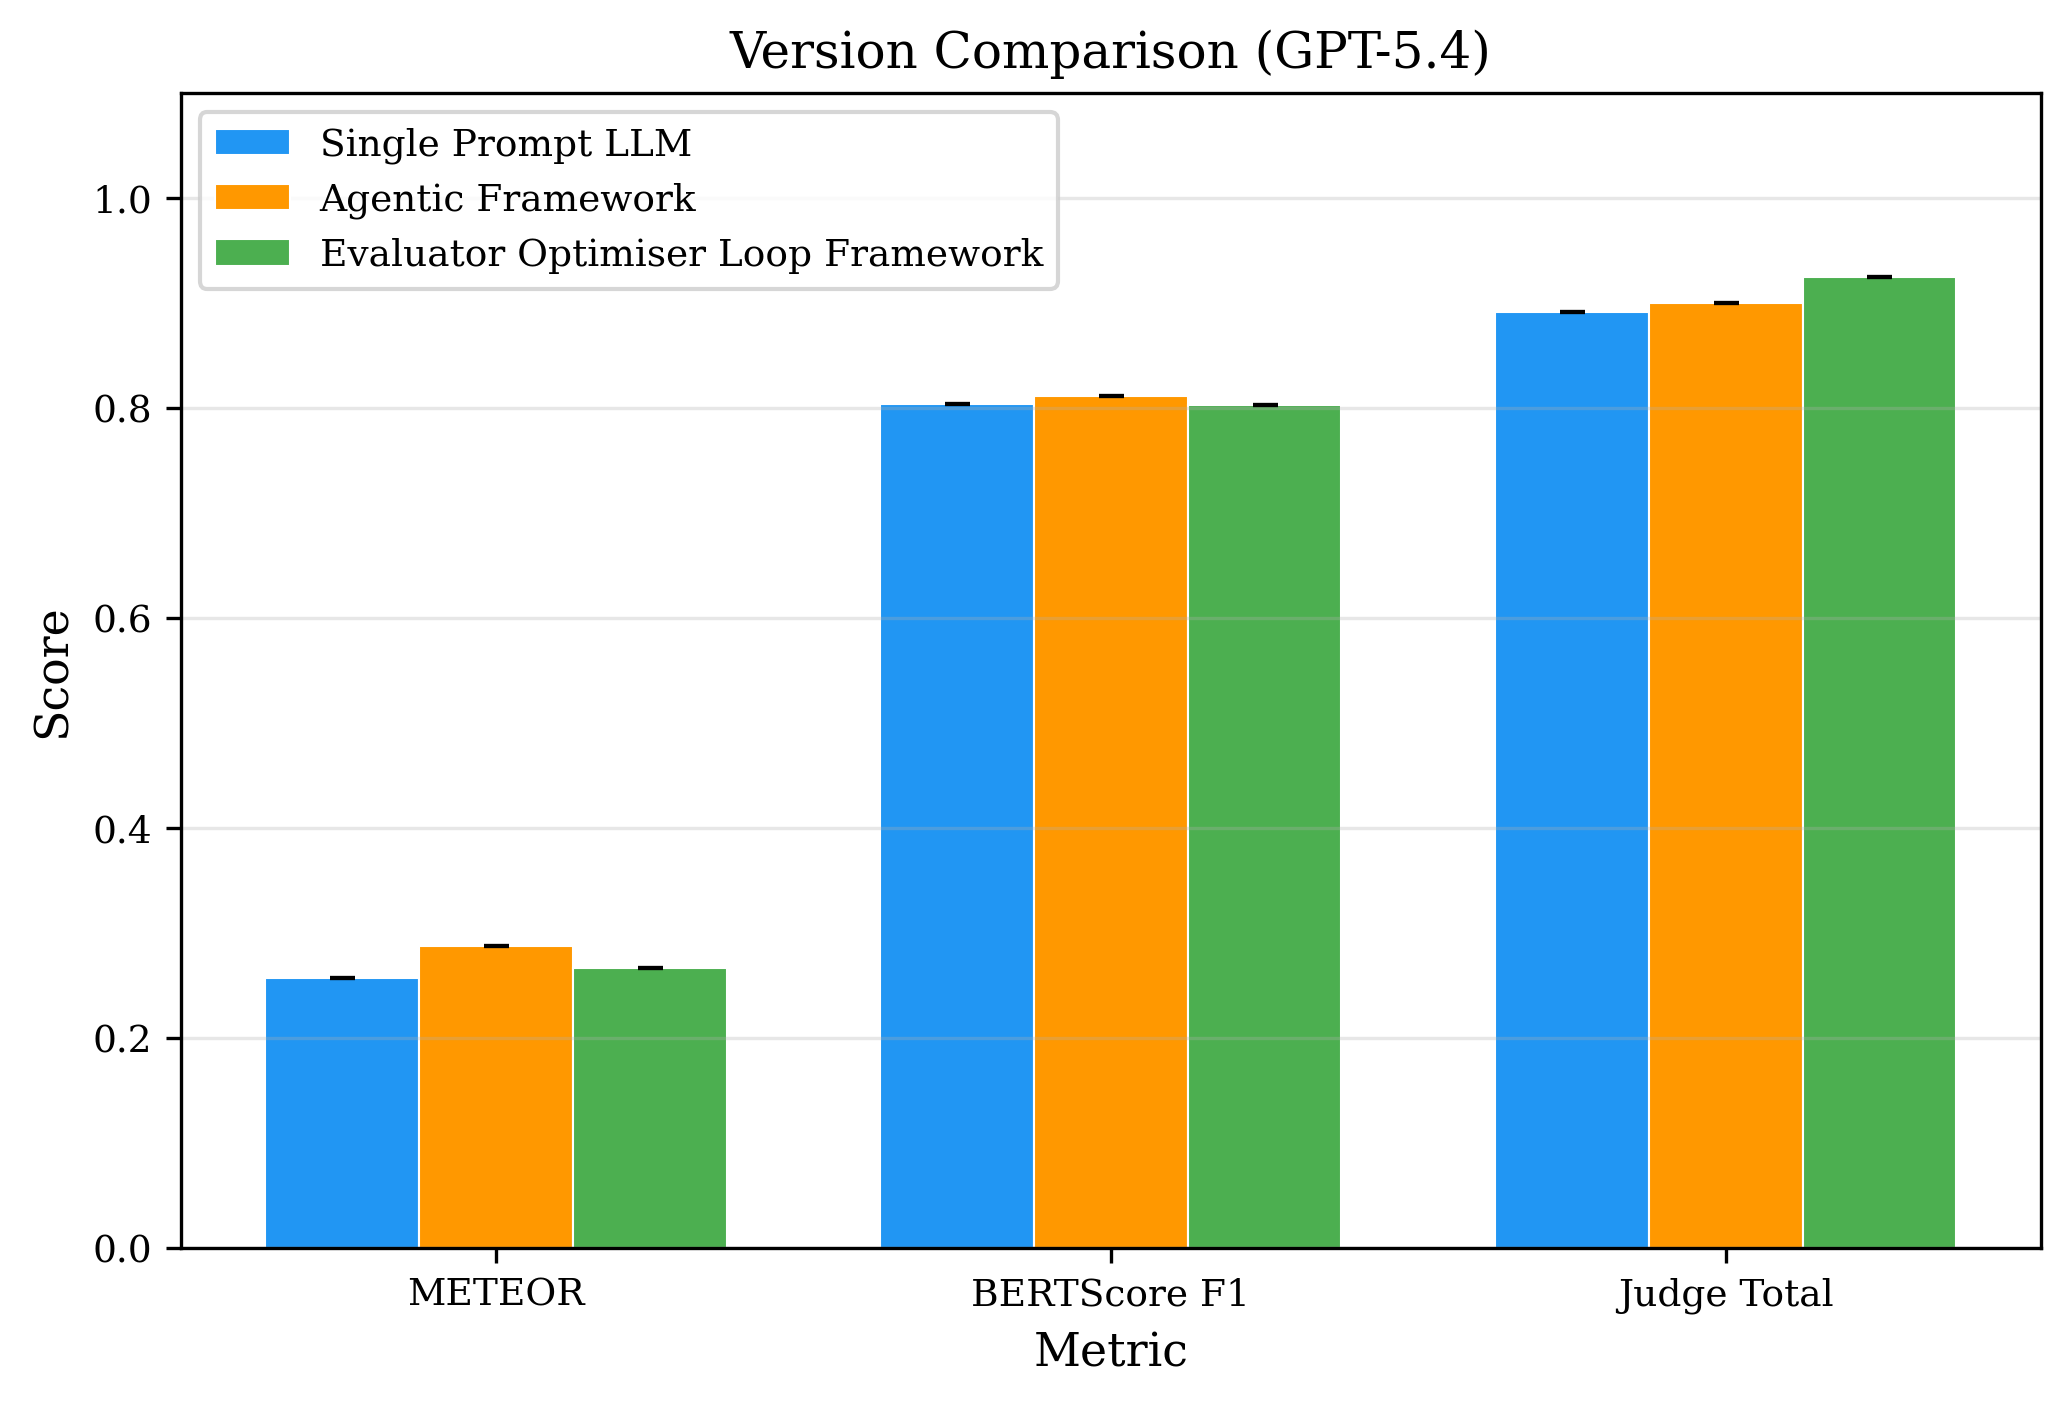
\includegraphics[width=0.85\textwidth]{../evaluation/results/charts/chart_version_grouped_bar.png}
    \caption{Grouped bar chart comparing METEOR, BERTScore F1, and judge total across the three framework variants. While surface-level lexical metrics fluctuate modestly, the judge score exhibits a clear monotonic increase as architectural sophistication is added.}
    \label{fig:version_grouped_bar}
\end{figure}

A notable observation is that METEOR does not increase monotonically with architectural quality. The full framework produces a slightly lower METEOR score (0.267) than the agentic draft (0.288), despite achieving a substantially higher judge total. This dissociation supports the Phase 1 finding that token-overlap metrics are insufficient evaluators for open-ended architecture generation tasks, where multiple correct solutions exist that share limited lexical surface with any single reference.

\section{Experiment 2: Cross-Model Comparison}

The second experiment holds the framework variant constant at the full Evaluator-Optimizer loop and varies the language model used for both the reasoning tier (supervisors, synthesizers) and the execution tier (domain architects and validators). Three frontier models are evaluated: GPT-5.4, Claude Sonnet 4.6, and Gemini 3.1 Pro.

\begin{table}[htbp]
\centering
\caption{Model Comparison Summary (Evaluator Optimiser Loop Framework, Aggregated Across Scenarios)}
\label{tab:model_summary}
\begin{tabular}{lccc}
\toprule
Metric & Claude Sonnet 4.6 & Gemini 3.1 Pro & GPT-5.4 \\
\midrule
METEOR & 0.191 & 0.294 & 0.267 \\
BERTScore F1 & 0.798 & 0.825 & 0.803 \\
Judge Total & 9.415 & 9.000 & 9.083 \\
\bottomrule
\end{tabular}
\end{table}

\begin{table}[htbp]
\centering
\caption{LLM Judge Dimension Breakdown by Model (Evaluator Optimiser Loop Framework)}
\label{tab:judge_breakdown}
\begin{tabular}{lccccccc}
\toprule
Model & Comp. & Accuracy & Security & Scalab. & Best Pr. & Specif. & Total \\
\midrule
Claude Sonnet 4.6 & 9.500 & 9.500 & 9.500 & 9.500 & 9.500 & 10.000 & 9.582 \\
Gemini 3.1 Pro & 9.000 & 9.000 & 9.000 & 9.500 & 9.000 & 9.000 & 9.083 \\
GPT-5.4 & 9.500 & 9.500 & 9.500 & 9.000 & 9.000 & 9.000 & 9.250 \\
\bottomrule
\end{tabular}
\end{table}

Table~\ref{tab:model_summary} presents the aggregate metrics. Claude Sonnet 4.6 records the highest judge total at 9.582, followed by GPT-5.4 at 9.250 and Gemini 3.1 Pro at 9.083. The per-dimension breakdown in Table~\ref{tab:judge_breakdown} reveals that Claude achieves perfect marks on Specificity (10.0) and uniform 9.5 across all remaining dimensions. GPT-5.4 matches Claude on Completeness, Technical Accuracy, and Security but trails by 0.5 points on Scalability and Best Practices. Gemini 3.1 Pro scores 9.0 on most dimensions with only a marginal advantage in Scalability (9.5).

\begin{figure}[h]
    \centering
    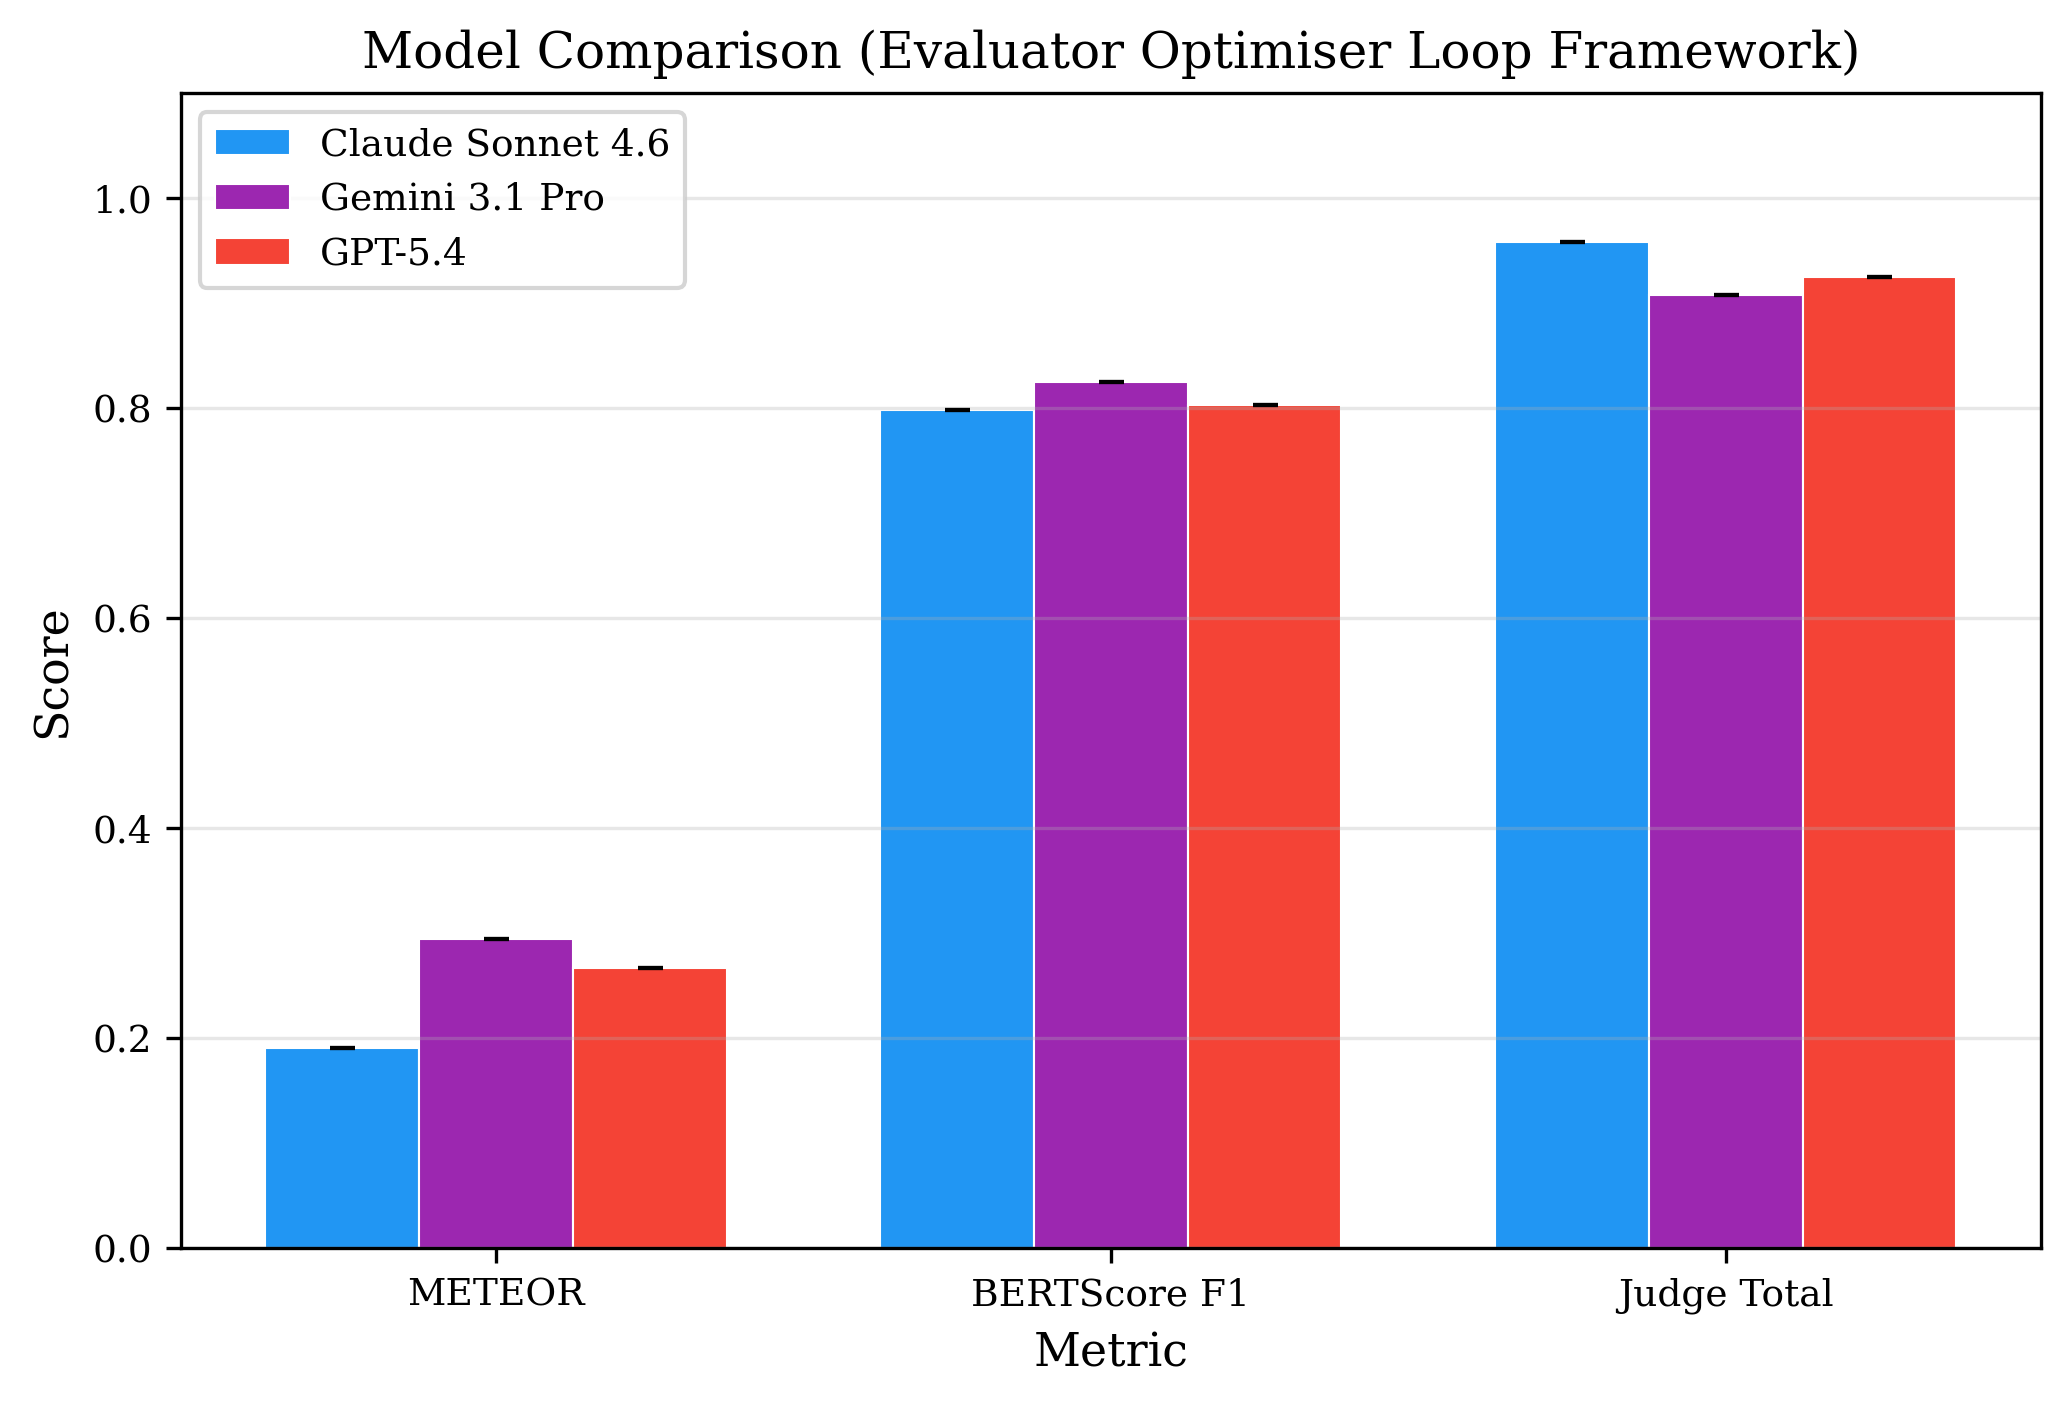
\includegraphics[width=0.85\textwidth]{../evaluation/results/charts/chart_model_grouped_bar.png}
    \caption{Grouped bar chart of METEOR, BERTScore F1, and judge total for each evaluated frontier model. Claude Sonnet 4.6 leads on the judge dimension while Gemini 3.1 Pro records the highest BERTScore F1.}
    \label{fig:model_grouped_bar}
\end{figure}

\begin{figure}[h]
    \centering
    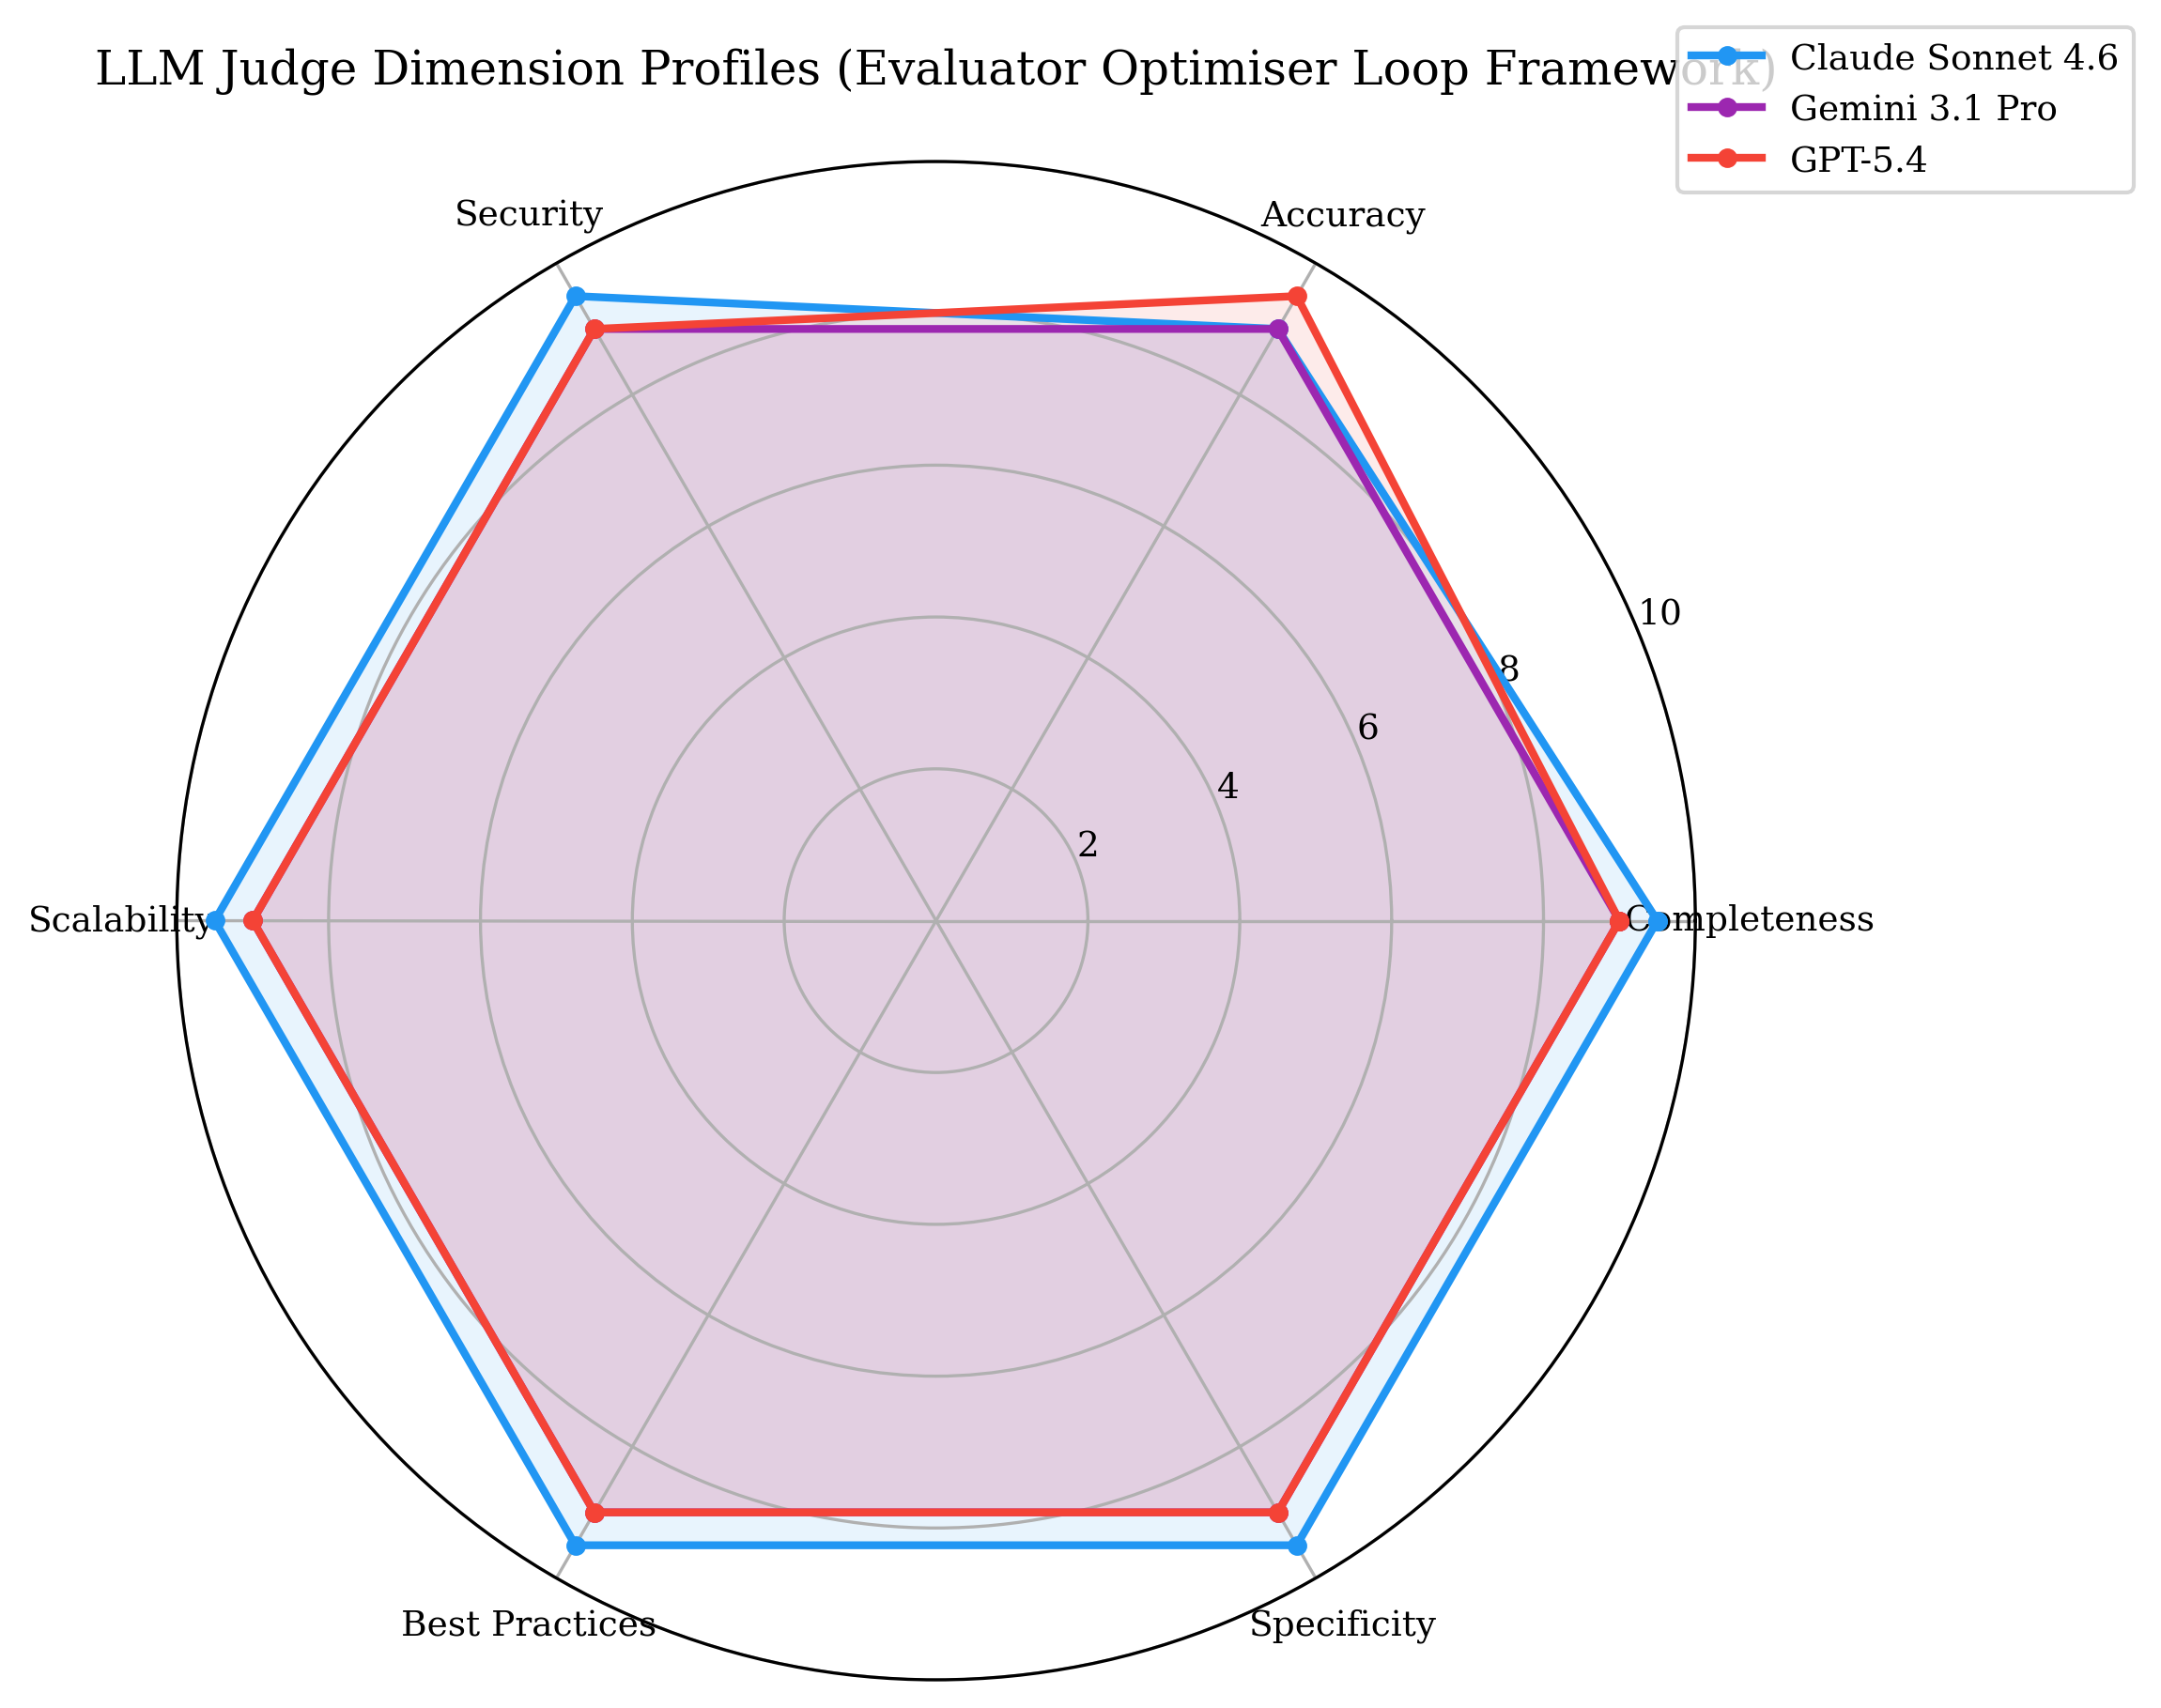
\includegraphics[width=0.75\textwidth]{../evaluation/results/charts/chart_model_radar.png}
    \caption{Radar chart of the six LLM judge dimensions for each model. Claude Sonnet 4.6 exhibits a near-regular hexagonal profile, indicating balanced performance without a pronounced weakness in any single dimension.}
    \label{fig:model_radar}
\end{figure}

An interesting inversion appears in the surface-level metrics: Gemini 3.1 Pro achieves the highest BERTScore F1 (0.825) and METEOR (0.294), yet scores lowest on the judge dimension. This pattern suggests that Gemini's outputs tend to be semantically closer to the human reference architectures in vocabulary and phrasing but are rated lower on deeper technical dimensions such as specificity and best practices. Conversely, Claude's architectures deviate more in wording from the reference texts (METEOR 0.191, BERTScore 0.798) while earning the highest expert assessment, reinforcing the argument that surface similarity and architectural quality are distinct properties.

\section{Interpretation and Discussion}

\subsection{Value of the Iterative Validation Loop}

The version ablation results affirm the core design hypothesis: an Evaluator-Optimizer loop that routes generated architectures through parallel domain validators and feeds structured feedback back into the generation subgraph produces measurably higher-quality outputs than either a single-prompt approach or an agentic system without validation. The 0.333-point gain in judge score between the baseline and the full framework, observed on a 10-point scale, corresponds to meaningful improvements in security specificity and operational correctness that would be consequential in a production cloud deployment.

\subsection{Effect of Cross-Encoder Reranking}

The two-stage RAG pipeline — dense vector retrieval followed by FlashRank cross-encoder reranking — concentrates the most contextually relevant documentation passages into the bounded context window presented to each domain agent. This selectivity appears to benefit precision-oriented dimensions (Technical Accuracy, Specificity) more than recall-oriented ones. Future ablation specifically targeting the reranking stage would quantify its isolated contribution.

\subsection{Judge Bias Caveat}

A methodological limitation warrants emphasis. The judge model \texttt{claude-sonnet-4-6} belongs to the same model family as one of the three test models. Research on LLM-as-a-Judge pipelines has documented a self-enhancement bias, wherein a model tends to rate outputs structurally similar to its own generation style more favourably \cite{zheng2024judging}. Consequently, Claude Sonnet 4.6's leading judge total of 9.582 should be interpreted with caution: some fraction of its advantage over GPT-5.4 (9.250) and Gemini 3.1 Pro (9.083) may reflect evaluator–subject alignment rather than a genuine quality differential. Rotating the judge model across multiple providers — a direction identified as future work — would provide a more robust cross-model ranking.

\subsection{Practical Considerations}

All three evaluated models produce architectures that are qualitatively sound and deployable, with judge scores exceeding 9.0 across the board. This high floor indicates that the framework's multi-agent decomposition, RAG grounding, and iterative validation collectively provide a strong quality scaffold that is relatively robust to the choice of underlying language model. In deployment scenarios where model availability or cost is a constraint, GPT-5.4 at 9.250 represents a strong default, while Gemini 3.1 Pro at 9.083 is a competitive alternative with favourable BERTScore characteristics.

\section{Summary}

Phase 2 evaluation establishes two primary findings. First, the Evaluator-Optimizer loop contributes a statistically meaningful uplift of 0.333 judge-score points over a single-prompt baseline, validating the iterative multi-agent design as the central architectural contribution of this work. Second, all three frontier models — GPT-5.4, Claude Sonnet 4.6, and Gemini 3.1 Pro — perform at a high level within the framework, with Claude recording the highest composite judge score while Gemini exhibits the strongest surface-level similarity to human reference architectures. The judge bias caveat prevents a definitive ranking between Claude and GPT-5.4 without independent multi-judge confirmation. These findings collectively demonstrate that the framework provides a robust, model-agnostic platform for automated cloud architecture generation and validation.
